% Created 2016-05-01 Sun 16:57
\documentclass[11pt]{article}
\usepackage[utf8]{inputenc}
\usepackage[T1]{fontenc}
\usepackage{fixltx2e}
\usepackage{graphicx}
\usepackage{grffile}
\usepackage{longtable}
\usepackage{wrapfig}
\usepackage{rotating}
\usepackage[normalem]{ulem}
\usepackage{amsmath}
\usepackage{textcomp}
\usepackage{amssymb}
\usepackage{capt-of}
\usepackage{hyperref}
\usepackage[portuguese, ]{babel}
\author{André Peric Tavares, Giulio Parva Denardi}
\date{\today}
\title{Projeto de Compiladores\\\medskip
\large Trabalho para a disciplina Compiladores na Universidade Federal do ABC sob orientação da Profa. Mirtha Lina Fernández Venero}
\hypersetup{
 pdfauthor={André Peric Tavares, Giulio Parva Denardi},
 pdftitle={Projeto de Compiladores},
 pdfkeywords={},
 pdfsubject={},
 pdfcreator={Emacs 24.5.1 (Org mode 8.3.3)}, 
 pdflang={Pt-Br}}
\begin{document}

\maketitle
\tableofcontents


\section{Introdução}
\label{sec:orgheadline1}
\textbf{negrito}
\emph{itálico}
\href{https://google.com}{google}
\hyperref[sec:orgheadline1]{link}
imagem:
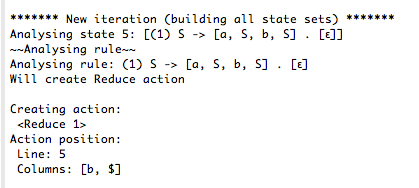
\includegraphics[width=.9\linewidth]{./media/Screenshot 2016-04-25 17.54.18.png}

\section{Objetivos}
\label{sec:orgheadline2}
\section{Justificativa}
\label{sec:orgheadline3}
\section{Funcionamento}
\label{sec:orgheadline12}
\subsection{Produção de cadeia vazia}
\label{sec:orgheadline4}
O cálculo dos conjuntos FIRST e FOLLOW exigem em diversos momentos saber se
um determinado não terminal produz \(\epsilon\). Por exemplo, considere a sequência
de símbolos \emph{ABC}. Queremos calcular FIRST(ABC). Sabemos que

\begin{center}
FIRST(ABC) = FIRST(A) \(\oplus\) FIRST(BCD)
\end{center}

e o resultado desta operação é somente FIRST(A) se \(A\) não produz \(\epsilon\) ou
FIRST(A) - \(\epsilon\) se \(\epsilon\) \(\in\) FIRST(A). Então é conveniente saber de
antemão quais símbolos produzem \(\epsilon\).

Para tanto, usa-se o método \texttt{buildAllNonTerminalsThatProduceEps} na classe
\texttt{Grammar}. O algoritmo utilizado é simples: primeiro, verifica-se todos os não
terminais que produzem diretamente \(\epsilon\), isto é, aqueles que têm uma regra
que produz \(\epsilon\) sem etapas intermediárias, como em \(A \rightarrow \epsilon\).

Em seguida, todas as regras são percorridas, e se todos os símbolos da parte
direita de uma regra produzem \(\epsilon\), então adicionamos o produtor dessa regra
à lista de não terminais que produzem \(\epsilon\). Todas as regras são percorridas
novamente até que nenhum símbolo novo tenha sido adicionado à lista de símbolos
que produzem \(\epsilon\). Em outras palavras, até que o ponto fixo seja atingido.

Por exemplo, considere a seguinte gramática:

\begin{center}
A \(\rightarrow\) BC \\
B \(\rightarrow\) \(\epsilon\) \\
C \(\rightarrow\) \(\epsilon\)
\end{center}

A tabela a seguir mostra o resultado desse algoritmo aplicado à gramática
anterior em cada iteração.

\begin{center}
\begin{tabular}{llll}
Produz \(\epsilon\)? & A & B & C\\
Iteração 1 & não & sim & sim\\
Iteração 2 & sim & sim & sim\\
Iteração 3 & sim & sim & sim\\
\end{tabular}
\end{center}

Na iteração 3, o conjunto de elementos que produzem \(\epsilon\) não mudou, e assim
o algoritmo termina.

O código é apresentado a seguir.

\begin{verbatim}
private final void buildAllNonTerminalsThatProduceEps() {
  Set<Symbol> nonTerminalsThatGenerateEps = new HashSet<Symbol>();

  // rules that directly generate eps
  for (Symbol nonTerminal : nonTerminals) {
    for (Rule rule : rules.get(nonTerminal)) {
      if (rule.producesEmptyString()) {
        nonTerminalsThatGenerateEps.add(nonTerminal);
      }
    }
  }

  // iterates until fp is found
  boolean newNonTerminalThatGeneratesEpsHasBeenFound = true;
  while (newNonTerminalThatGeneratesEpsHasBeenFound) {
    newNonTerminalThatGeneratesEpsHasBeenFound = false;
    int setSizeBeforeIteration = nonTerminalsThatGenerateEps.size();

    for (Symbol nonTerminal : nonTerminals) {
      for (Rule rule : rules.get(nonTerminal)) {
        // verifies if all symbols from rule produce eps
        List<Symbol> production = rule.getProduction();
        boolean allSymbolsFromProductionProduceEps;
        allSymbolsFromProductionProduceEps = production
            .stream()
            .allMatch(symbol -> nonTerminalsThatGenerateEps.contains(symbol));

        // if so, add it to set
        if (allSymbolsFromProductionProduceEps) {
          nonTerminalsThatGenerateEps.add(nonTerminal);
        }
      }
    }

    // verifies whether some non terminal has been added to set
    int setSizeAfterIteration = nonTerminalsThatGenerateEps.size();
    if (setSizeBeforeIteration != setSizeAfterIteration) {
      newNonTerminalThatGeneratesEpsHasBeenFound = true;
    }
  }

  // initialise Map
  Map<Symbol, Boolean> producesEps = new HashMap<Symbol, Boolean>();
  for (Symbol nonTerminal : nonTerminals) {
    producesEps.put(nonTerminal, nonTerminalsThatGenerateEps.contains(nonTerminal));
  }
  for (Symbol terminal : terminals) {
    producesEps.put(terminal, false);
  }

  this.nonTerminalsToProducesEps = producesEps;
}
\end{verbatim}

\subsection{Representação dos conjuntos FIRST e FOLLOW}
\label{sec:orgheadline5}
Uma das principais funcionalidades do programa deste trabalho é não só calcular
os conjuntos FIRST e FOLLOW, mas fazer isso apresentando as etapas
intermediárias, fazendo com que o usuário veja cada passo do algoritmo. Isso faz
com que o cálculo desses conjuntos não seja o mais eficiente possível, pois
precisamos lidar também com o \emph{output} sem pular nenhuma etapa.

Para isto, criamos classes \texttt{First} e \texttt{Follow}. Estas classes têm atributos que
indicam a \emph{representação} do conjunto dado em termos de outros conjuntos.

Por exemplo, considere os seguintes atributos da classe \texttt{Follow}:

\begin{verbatim}
private Set<Symbol> firstSets;
private Set<Symbol> firstSetsWithoutEps;
private Set<Symbol> followSets;
private Set<Symbol> terminals;
private boolean hasEOF;
\end{verbatim}

Suponha que um objeto dessa classe tenha as seguintes atribuições (aqui em
notação de teoria dos conjuntos):

\begin{center}
firstSets = \{A\} \\
firstSetsWithoutEps = \{B, C\} \\
followSets = \{D\} \\
terminals = \{a, b\} \\
hasEOF = true \\
\end{center}

Então esse conjunto seria

\begin{center}
FIRST(A) \(\cup\) (FIRST(B) - \(\epsilon\)) \(\cup\) (FIRST(C) - \(\epsilon\)) \(\cup\) FOLLOW(D)
\(\cup\) \{a\} \(\cup\) \{b\} \(\cup\) \{\$\}
\end{center}

Ambas as classes têm o método \texttt{toString} sobrescrito para exibir essa
representação como mostrado acima e um método \texttt{getAllElements} que coleta
todos os elementos vindos da união dos conjuntos.

\subsection{Cálculo dos conjuntos FIRST e FOLLOW}
\label{sec:orgheadline6}
De maneira semelhante à computação de todos os não terminais que geram \(\epsilon\),
o cálculo dos conjuntos FIRST e FOLLOW consiste, em essência, em iterar até
encontrar um ponto fixo.

Note que a aplicação direta da definição de FIRST e FOLLOW não funciona, pois
ela falharia no caso de definições recursivas que são dependentes entre
si. Por exemplo, considere o caso em que FIRST(A) = FIRST(B) e FIRST(B) =
FIRST(A). Para calcular FIRST(A), calcula-se FIRST(B). Mas FIRST(B) é FIRST(A),
o que resulta num \emph{loop} infinito. Em vez disso, começamos com todos os
conjuntos FIRST setados para \(\emptyset\), e a cada iteração atualizamos todos os
conjuntos até atingir um ponto fixo. 

O código a seguir mostra a implementação desse algoritmo para o cálculo dos
conjuntos FIRST.

\begin{verbatim}
public final void buildAllFirstSets() {

  // Initialize set
  // omitido

  // Get description of each first set
  Map<Symbol, First> firstSetDescriptions = buildAllFirstSetDescriptions();

  // Iterate until fixed point is found
  boolean someFirstSetHasChanged = true;
  while (someFirstSetHasChanged) {
    StringBuilder iterationSb = new StringBuilder();
    iterationSb.append("New iteration (building first sets)\n");
    someFirstSetHasChanged = false;

    // Copy elements from old first sets to new first sets
    // omitido

    // Updates, possibly getting new elements
    for (Symbol nonTerminal: nonTerminals){
      iterationSb.append(String.format("Updating First(%s)\n", nonTerminal));
      First firstDescription = firstSetDescriptions.get(nonTerminal);
      iterationSb.append(String.format("First(%s) = %s\n", nonTerminal, firstDescription));
      int numElementsBefore = firstSetsBeforeIteration.get(nonTerminal).size();
      firstSetsAfterIteration.get(nonTerminal).addAll(firstDescription.getAllElements(firstSetsBeforeIteration));
      iterationSb.append(String.format("Adding elements: %s\n", firstDescription.getAllElements(firstSetsBeforeIteration)));
      int numElementsAfter = firstSetsAfterIteration.get(nonTerminal).size();
      if (numElementsBefore != numElementsAfter){
        someFirstSetHasChanged = true;
      }
    }

    iterationSb.append(String.format("All elements form first sets before iteration: %s\n", firstSetsBeforeIteration));
    iterationSb.append(String.format("All elements form first sets after iteration: %s\n\n", firstSetsAfterIteration));

    firstSetsBeforeIteration = firstSetsAfterIteration;
  }
  this.firstSets = firstSetsBeforeIteration;
}
\end{verbatim}

O cálculo dos conjuntos FOLLOW é bastante semelhante, e por isso é omitido.

\subsection{{\bfseries\sffamily TODO} LL}
\label{sec:orgheadline7}

\subsection{SLR}
\label{sec:orgheadline11}
\subsubsection{Ações}
\label{sec:orgheadline8}

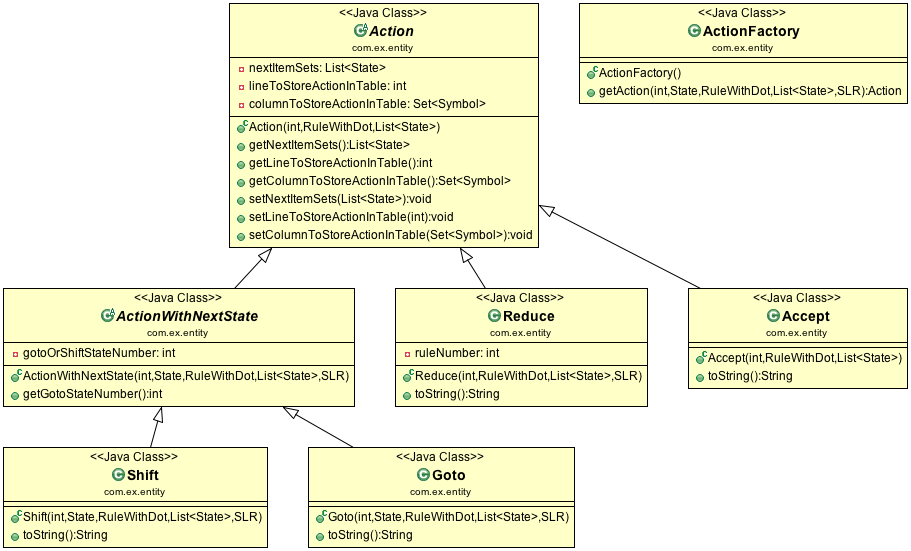
\includegraphics[width=.9\linewidth]{./media/actions.png}

\subsubsection{Regras}
\label{sec:orgheadline9}
\subsubsection{Algoritmo}
\label{sec:orgheadline10}
\section{Conclusão}
\label{sec:orgheadline13}
\section{Adendo - notas sobre algumas decisões de \emph{design}}
\label{sec:orgheadline14}
\section{Referências Bibliográficas}
\label{sec:orgheadline15}
\end{document}